\documentclass[sotsuron]{jcsie}
\usepackage[dvipdfmx]{graphicx}
\usepackage{float}
\usepackage{listings}

\lstset{
  basicstyle={\ttfamily}, 
  identifierstyle={\small}, 
  commentstyle={\smallitshape}, 
  keywordstyle={\small\bfseries}, 
  ndkeywordstyle={\small}, 
  stringstyle={\small\ttfamily}, 
  frame={tb}, 
  breaklines=true, 
  columns=[l]{fullflexible}, 
  numbers=left, 
  xrightmargin=0zw, 
  xleftmargin=3zw, 
  numberstyle={\scriptsize}, 
  stepnumber=1, 
  numbersep=1zw, 
  lineskip=-0.5ex
}

\title{ライブストリーミングに対応した分散ハッシュテーブルの設計と実装}
\etitle{Design and Implementation of Distributed Hash Table for Live Streaming}
\author{沈 嘉秋}
\eauthor{Yoshiaki Shin}
\id{T18I917F}
\keywords{P2P, 分散ハッシュテーブル}
\ekeywords{P2P, Distributed Hash Table}

\begin{document}
\maketitle
\emaketitle
\pagenumbering{roman}
\begin{abstract}    
分散ハッシュテーブルはファイル共有サービス等に応用され, 
すでに普及している一方で, 
近年はブロックチェーンの関連技術としても注目を集めている.
%
分散ハッシュテーブルの中でもKademlia
はその実装の容易さとノードの出入りに対する耐性の強さから
実用的なサービスへの応用が可能であり, 
多くのサービスで採用されている.
%
近年, ライブストリーミングサービスの需要が高まっている
一方で配信プラットフォームの事業者への依存が強く
サービス利用者の立場は弱いものとなっている.
そこで本論文では分散的なライブストリーミングサービスの基盤となる
システムをKademliaを元に実装し, その評価を行った.
%
Kademlia上で単純にライブストリーミングの実装を行う場合, 
非効率的な通信が発生するが, 本論文の手法では, 
Kademliaネットワークを階層化することで
非効率的な通信を削減することが可能となった.
%
結果, 分散的なライブストリーミングサービスの実装への
足がかりを作ることが出来た.
\end{abstract}
\begin{eabstract}
Distributed hash tables have been applied to file sharing services, 
and have already become widespread.
In recent years, they have also attracted attention as 
blockchain-related technologies.
%
Among the distributed hash tables, 
Kademlia can be applied to practical services 
and is adopted by many services 
because of its ease of implementation and resistant against churn.
%
In recent years, demand for live streaming services has been increasing.
On the other hand,
the dependence of distribution platforms on business operators is strong, 
and the position of service users is weak.
%
In this paper, we implement and evaluate the underlying system 
of a live streaming service based on Kademlia.
%
The simple implementation of live streaming in 
Kademlia reduces communication efficiency, 
but in this paper we can reduce inefficient communication by 
customize Kademlia networks.
%
As a result, we were able to create a foothold for implementing 
a distributed live streaming service.
\end{eabstract}
\setcounter{tocdepth}{2}
\tableofcontents
\pagenumbering{arabic}

% ---------------------------------------------------------------------

\chapter{序論}
\section{背景}
\label{sec:haikei}
近年, P2Pネットワーク技術がブロックチェーンなどによって再び注目を集めている.
最近ではブロックチェーン流行以前に研究されていた
P2Pネットワーク技術を利用した分散型ファイル共有システムと
ブロックチェーンを組み合わせて開発されたサービスも登場している
\cite{BitTorre1:online}.
分散型ファイル共有サービスは分散ハッシュテーブルという技術を用いて
実装されることがあり, 分散型ファイル共有サービスの中でも
利用者の特に多いBitTorrent\cite{BitTorre59:online}
はKademlia\cite{maymounkov2002kademlia}\cite{高野祐輝2010nat}
という分散ハッシュテーブルを用いて開発されている.

分散型ファイル共有サービスはこれまで, 膨大なサーバリソースを持つ
大企業などでなければ実現できなかった, 大規模かつ, 高速な
ファイル共有を実現した.

近年の家庭用ネットワークやモバイルネットワークの環境改善に伴い
Youtube Live\footnote{https://www.youtube.com/live} や 
Twitch\footnote{https://www.twitch.tv} 
といった高いスループットが要求される動画ライブストリーミングサービス
が急速に普及してきている.
しかし, これらのサービスは膨大なサーバリソースを持つ大企業
や大企業の提供するクラウド環境を利用するなどしなければ実現が
難しく,  プラットフォーム事業者やクラウド事業者への依存が強く, 
サービス利用者の立場は弱いものとなっており不健全な状態にある.
ファイル共有サービスが分散型ファイル共有サービスによって, 
リソースの分散化に成功したようにライブストリーミングサービスも
リソースの分散化が行われることが望ましいと考えられる.

\section{目的}
第\ref{sec:haikei}節で述べたように, 
ライブストリーミングサービスの分散化には意義がある.
そこで本論文では, 分散型の動画ライブストリーミングサービスの基盤
となるシステムを, Kademliaという分散ハッシュテーブルをベースに実装する.

分散ハッシュテーブルの中でもKademliaはその実装の容易さと
高いchurn耐性\footnote{ノードの出入りに対する耐性の強さ}
を持つことから実用的なサービスへの応用が可能である.
しかし, その一方でKademlia上で単純にライブストリーミングの実装を行う場合, 
高頻度に追加されるストリームのチャンクデータの共有を
スケールさせることは困難である.
そのため, Kademliaを更に構造化したLayeredKadという手法を提案する.
LayeredKadは他の分散ハッシュテーブルと同じように
データのIDに対応するデータをP2Pネットワーク上で探索し
入手することができる.

LayeredKadがWebブラウザとNode.jsで動作するライブラリとなるように開発を行う.
ライブラリができるだけ多くのプラットフォームで動作するようにするために
P2P通信箇所にWebRTC \cite{WebRTCHo80:online}を用いる.

完成したライブラリを用いてWebブラウザ上で動作する
ライブストリーミングの配信と視聴を行うサンプルプログラム
を作成し動作確認を行う.
LayeredKadのライブラリを用いたベンチマークプログラムと
Kademliaを用いたベンチマークプログラムをNode.js上で実行し
その性能や性質の比較検証を行う.

\section{本論文の構成}
本論文ではTypeScript\footnote{https://www.typescriptlang.org}
というプログラム言語を用いて研究を行っている.
そのため, 本文中に登場するコードサンプルはすべてTypeScriptによるものである.
本研究のソースコードはGithub上のリポジトリ\cite{shinyosh38:online}で
GPLv3\footnote{https://www.gnu.org/licenses/gpl-3.0.html}
ライセンスで公開している.

% ---------------------------------------------------------------------

\chapter{関連事例}
\section{分散ハッシュテーブル}
分散ハッシュテーブルとは, 分散型のkey-valueストアを実現する手法であり, 
あるデータとそのデータのハッシュ値をペアとしたハッシュテーブルを
P2Pネットワーク上で複数のノードによって分散的に実装する技術である.
複数のノードにデータを分散配置をするため適切な構造化を行う必要がある.
構造化には様々な手法が存在し, 
ChordやKademliaといったさまざまな実装が存在する.

\section{Kademlia}
Kademliaは分散ハッシュテーブルの一種である.
高いChurn耐性を持つため, 実用的なP2Pアプリケーションに多く利用されている.

本研究ではKademliaをTypeScriptで実装した.
Node.jsとChrome上で動作するようにするためにP2P通信部分にWebRTCを利用した.

\subsection{採用例}
Kademliaは高いChurn耐性を持ちながら, 実装も容易であるため, 
多くの分散型のサービスで利用されている.
ここでは, Kademliaを利用している有名なサービスを幾つか紹介する.
サービスの紹介を表\ref{table:kademlia-services}に示す.
\begin{table}[H]
	\caption{Kademliaを利用したサービス}	
	\centering
	\label{table:kademlia-services}
	\begin{tabular}{|l|l|}
		\hline
		サービス名 & 使用箇所 \\ 
		\hline
		Torrent         &              
		\begin{tabular}{l}
		magnetURLという機能を用いてファイルをダウンロードする際に\\
		目的のファイルを持っているノードを探索するのにKademliaを用いている.\\
		Torrentはアクティブユーザと転送量という点で見ると\\
		世界で最も成功したP2Pのシステムであり, \\
		そのシステムにKademliaはおおいに貢献していると言える.\\
	\end{tabular}\\ \hline
	Ethereum &
	\begin{tabular}{l}
		Node Discovery Protocol v4 というノードの探索プロトコルに用いられている. 
	\end{tabular}\\ \hline
	IPFS     &
	\begin{tabular}{l}
		IPFSとは複数のノードが協調して一つの大きなストレージ                       \\
		またはHTTPの置き換えとして機能することを目的としているシステムある. \\
		IPFSはKademliaをベースとして開発されている                                          \\
	\end{tabular}\\ \hline
	\end{tabular}
\end{table}

\subsection{Kademliaのアルゴリズム}
\subsubsection{ノードIDとKey}
Kademliaでは個々のノードに固有のノードIDが割り振られており, 
このIDを元にルーティングを行う.このノードIDは160bitと定義されている.
ノードIDの決定方法は, ランダムな値にsha1というハッシュ関数を適用し, 
160bitの値を取り出すのが一般的である.
また, ハッシュテーブルに保存するValueと対になるKeyも
160bitと定義されている.

\subsubsection{経路表}
分散ハッシュテーブルのアルゴリズムによって
ノードを管理する経路表の形は様々である.
例えば, Chordという分散ハッシュテーブルの場合は環状の経路表を持っている.
Kademliaはk-bucketsという160個のk-bucketからなる二分木状の経路表を持っている.
一つのk-bucketにはK個(本研究では20個)のノードが登録でき, 
自身のノードとの距離に応じたk-bucketにそれぞれのノードが登録されていく.
ノード間の距離は2進数のノードID同士をXORで掛け合わした結果を
10進数に戻した値を用いる.

\subsubsection{プロトコル}
Kademliaには4種類の通信問い合わせがある.名称と内容についてまとめる.
\begin{itemize}
	\item {PING}\\
		  対象のノードがオンラインかどうかを問い合わせる.\\
	\item {FIND\_NODE}\\
	      自身のk-bucketsのうち最もKeyにXOR距離の近いノードに
	      自身のノードIDと距離が近い上位K個のノードの情報を送らせる.\\
	\item {STORE}\\
	      対象ノードにValue, Keyの組を保持させる.
		  保持させる際のルールは, 
		  Keyに対してFindNodeをk-bucketsのKeyに対するXOR距離が近い
		  上位K個のノードが固定されるまで繰り返し実行し
		  k-bucketsにKeyにできるだけXOR距離が近いノードが入るように
		  k-bucketsの最適化を行う.
		  次に自身のk-bucketsから最もKeyにXORの距離が近いノードを近い順に
		  K個選択し, そのノードらにValue, Keyの組を与える.\\	
	\item {FIND\_VALUE}\\
	      自身のk-bucketsのうち最もKeyにXOR距離の近いノードに
	      Keyに対応するValueを持っているか問い合わせる.
	      問い合わせられたノードはValueを持っている場合はそのValueを, 
	      持っていない場合は問い合わせられたノード自身のk-bucketsのうち, 
	      keyにXOR距離が近い上位K個のノードの情報を返す.\\
\end{itemize}

\subsubsection{経路表の更新}
ノードは4つのプロトコルのいずれかのメッセージを受け取った際に
送信元が該当するk-bucketの中にあった場合そのノードをk-bucketの末尾に移す.
送信元が該当するk-bucketの中に存在しないせず, k-bucketがすでに満杯な場合, 
そのk-bucket中の先頭のノードがオンラインかどうかをPINGで確認する.
オンラインなら先頭のノードを残し, 
そうでなければ送信元の新しいノードをk-bucketに追加する.
こうすることで長時間オンラインになっているノードが優先的にk-bucketに残るため, 
ネットワークの安定性が増す.

\subsubsection{ノードの新規参加}
新規参加するノードは, 
まず接続先のノードに対して自身のノードIDをKeyとしてFIND\_NODEを行う.
問い合わせを受けたノードは送信元のKeyに近い最大K個のノードの情報を
送信元のノードに返す.
そうすることで, 新規参加するノードはまず最大K個のノードに接続される.
このあと, さらに自身のk-bucketsのうち最も自身のノードIDに
XOR距離が近い上位K個のノードに対し自身のノードIDをKeyとしたFIND\_NODEを
自分のIDに対するXOR距離が近い上位K個のノードが固定されるまで繰り返す.

\subsubsection{ノードの離脱}
何もしない

\section{WebRTC}
本論文では, 
ブラウザとネイティブ環境の両方で動作するP2P通信手法が要求される.
そこで, その要求を満たす, WebRTCをP2P通信部分に使用した.

WebRTCとはW3Cが提唱するリアルタイム通信用の規格で,プラグイン無しで
ウェブブラウザ間のボイスチャット,ビデオチャット,ファイル共有
ができる.
WebRTCはブラウザ向けの規格として誕生したが,
現在では,Windows, Linux, Mac, AndroidやiOSといったネイティブ環境で
動作するlibwebrtc\footnote{https://webrtc.googlesource.com/src}
などの実装が公開されている.
WebRTCにはNAT越えを実現するために
ICE\cite{rosenberg2010interactive}という仕組みを採用している.

WebRTCには任意のデータを通信するためのDataChannelと
音声や動画などのメディアを通信するためのMediaChannelの
2種類の通信方法が存在する.本研究ではKademliaの実装における
UDPの代換えとしてWebRTCを用いるため, 通信方法にDataChannel
を利用する.

\subsection{NAT越え}
NATとは,
インターネットプロトコルによって構築されたコンピュータネットワークにおいて,
パケットヘッダに含まれるIPアドレスを,別のIPアドレスに変換する技術である.
プライベートネットワーク環境下でプライベートIPアドレスを持つホストから,
グローバルIPアドレスを持つゲートウェイを通して,
インターネットにアクセスする際に,プライベートIPアドレスを
グローバルIPアドレスに変換するために利用されることが多い.
モバイルネットワークにおいてはキャリアグレードNATが用いられている.
そのため,スマートフォン間でP2P通信を行うためには,
NAT越えを行う必要がある.
本研究ではWebRTCを用いてNAT越えを行う.
WebRTCではICEの情報をやり取りすることで,NAT越えを行っている.
ICEとは通信可能性のある通信経路に関する情報を示し,
文字列で表現される.次のような複数の経路を候補とする.
\\\\
・P2Pによる直接通信\\
・STUNによる,NAT通過のためのポートマッピング\\
・TURNによる,リレーサーバーを介した中継通信\\

STUN\cite{wing2008session}とは,
P2P通信を行うアプリケーションにおいて,
NAT越えの方法の1つとして使われる標準化されたインターネットプロトコルである.
STUNプロトコルは,アプリケーションがNATの存在と種類を発見し,
リモートホストへのUDP接続に
NATが割り当てたグローバルIPアドレスとポート番号とを得ることを許す.
STUNプロトコルが動作するには,インターネット上にSTUNサーバが存在する必要がある.

TURN\cite{matthews2010traversal}とは,
NATやファイアウォールを超えた通信することを補助するための
インターネットプロトコルである.
TURNが一番役立つのは,TCP, UDPを使って
対象型NAT装置により隠蔽されたプライベートネットワークに
接続されたクライアントで利用する場合である.

本研究ではGoogleが無料公開しているSTUNサーバ\footnote{stun.l.google.com:19302}
を用いている.本研究ではTURN
サーバが無くともP2P通信が疎通する環境で検証を行うため, 
TURNサーバは利用していない.

\subsection{シグナリング}
WebRTCでは,SDPとICE Candidateの二つの情報を端末間で交換することによって
P2P通信が開始される.このSDP等を交換する作業をシグナリングと言う.
シグナリングを行うためにはSDPとICE Candidateを交換する必要がある.
シグナリングにはTrickle IceとVanilla Iceの2つの方法がある.
本研究ではVanilla Iceというシグナリング手法を用いる.
Vanilla Iceは,実装が容易である,
シグナリングのための通信回数が少ないというメリットがある一方,
P2P接続の完了にかかる時間がTrickle Iceより長くなる傾向がある.
Vanilla Iceの手順について説明する.
Vanilla Iceの概要図を図\ref{fig:signaling}に示す.
\begin{figure}[H]
	\centering
	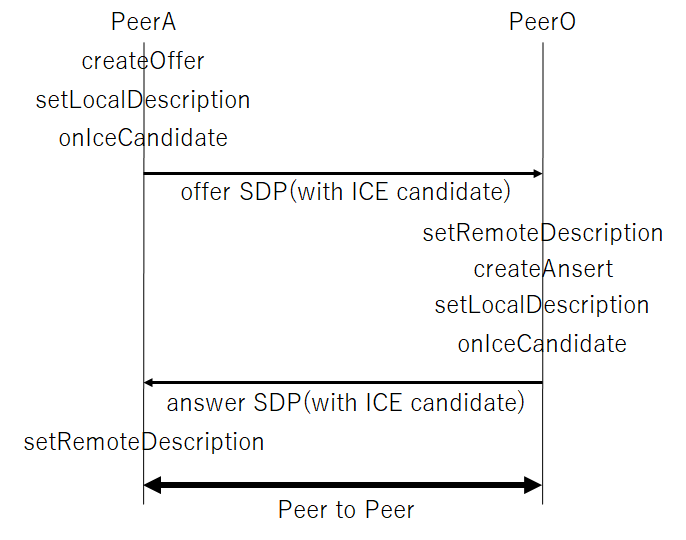
\includegraphics[width=10cm]{./assets/image/signaling.png}
	\caption{シグナリング}
	\label{fig:signaling}
\end{figure}
PeerAがcreateOfferを行いoffer側のSDPの作成準備を行う.
次にsetLocalDescriptionでSDPを作成し,
ICE candidateのリストアップを行う.
ICE candidateのリストアップが完了すると,
ICE candidateをoffer側のSDPの中に含ませて,PeerOへ送る.
PeerOはPeerAのoffer側のSDPをsetRemoteDescriptionで受け取り,
createAnswerでanswer側のSDPの作成準備を行う.
setLocalDescriptionでSDPを作成し,ICE candidateのリストアップを行う.
ICE candidateのリストアップが完了するとICE candidateを
answer側のSDPの中に含ませて,PeerAへ送る.
PeerAはPeerOのanswer側のSDPをsetRemoteDescriptionで受け取りP2P接続が完了する.

% ---------------------------------------------------------------------

\chapter{提案手法}
\section{概要}
本章では, Kademliaをベースに改良を施し, 
効率的にストリーム形式のデータを共有できるようにした
システムであるLayeredKadを提案する.
LayeredKadが分散型のライブストリーミングサービスの開発基盤に
なれるような性能を発揮できることを目指す.

Kademliaはデータを共有する際に, 
FindNodeを繰り返し実行し, k-bucketsを最適化する.
その際に, ネットワーク上の不特定多数のノードと通信した上, 
最大でK個の不特定なノードにデータを保存することになる.
そのためKademliaで連続的なストリーム形式のデータを共有する場合, 
個々のストリームのチャンクデータをネットワーク全体の
不特定多数のノード("$ チャンク数 \times K $"個)に保存することになる.
ライブ映像のようなチャンクの生成周期が非常に短く, 
高頻度にデータ共有する必要がある場合, Kademliaでは, 
ネットワーク全体に対して連続的にその都度, 負荷をかけることになり, 
データ共有の効率が非常に悪化することが予測される.

そこでLayeredKadでは共有するデータごとに別のKademliaネットワークを作成し
ネットワーク自体のスコープをデータごとに区切ることで, 
データの共有がネットワーク全体への負荷にならないようにし, 
ストリームデータのような連続的なデータでも効率よく共有できるようにする.

本手法では, 共有するデータの情報をメタデータとして, 
全ノードが参加するKademliaネットワーク上で共有する.
このメタデータを共有するネットワークをMainNetと定義する.
MainNet上でメタデータの実体データの共有を目的とするノード同士で
さらに別のKademliaネットワークを構築し, メタデータの情報に従い
メタデータに対応する実体データの共有を行う.
この実体データを共有するネットワークをSubNetとする.
MainNetとSubNetの関係を図\ref{fig:image}
に示す.

\begin{figure}[H]
	\centering
	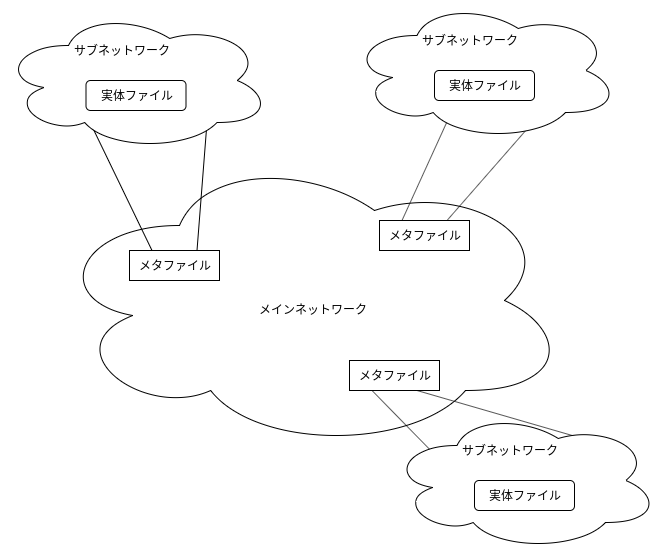
\includegraphics[width=10cm]{./assets/image/image.png}
	\caption{MainNetとSubNet}
	\label{fig:image}
\end{figure}

LayeredKadにおける幾つかの用語はBitTorrentのRFC\cite{bep0000r38:online}
の影響を受けている.

\section{Kademliaの拡張}
KademliaのStoreは単にValueとKey(Valueのハッシュ値)のペアしか情報を
持たない.
しかし, ストリームデータを扱う際にチャンクデータ同士の
関係性を表すためにはValueとKeyだけでは情報が不足する.
そのためLayeredKadのKademliaではValueとKeyのペアに対し
任意の文字列をアノテーションすることを許可する拡張を行う.
このアノテーションは現状ストリームデータの共有にのみ用いられる.
\\\\
拡張されたStoreの型定義を示す.
\begin{lstlisting}
	type Store = 
		(key: string, value: any, msg?: string) => void
\end{lstlisting}
KeyはValueのsha1ハッシュ値である必要があるが, 
msgはアノテーションであり, 任意の文字列を取ることができる.

\section{ストリームデータ}
\subsection{ストリームデータの保存}
ストリームデータは動的に生成される複数のチャンクデータから成り立つ.
LayeredKadでは一つのID(最初のチャンクのハッシュ値)
から全チャンクデータを探索できるようにする必要がある.
そのため, チャンクデータをKademlia上に保存する際には, 
そのチャンクデータ(便宜上chunkとする)の次に生成される
チャンクデータ(便宜上next chunkとする)が生成されるのを待ち, 
next chunkのハッシュ値をKey-Valueのmsgアノテーションとする.
ストリーミングを終了する際にはmsgにハッシュ値ではなく, 
"complete"文字列を与える.
チャンクデータを保存する様子を図\ref{fig:streamdata}に示す.
\begin{figure}[H]
	\centering
	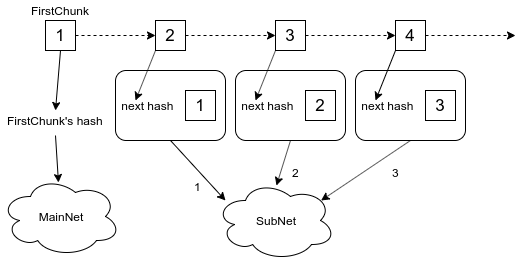
\includegraphics[width=10cm]{./assets/image/stream.png}
	\caption{ストリームデータの保存}
	\label{fig:streamdata}
\end{figure}

\subsection{ストリームデータの探索}
\label{sec:subscribe-stream}
図\ref{fig:subscribe-stream}のようにFirstChunkのKeyを元に
探索したValueのmsgアノテーションを辿ることで, ストリームデータ
を動的に継続的に取得できるようになっている.
msgの中がハッシュ値ではなく"complete"文字列なら, ストリームデータ
が終了したとみなし, ストリームの観測を終了する.

\begin{figure}[H]
	\centering
	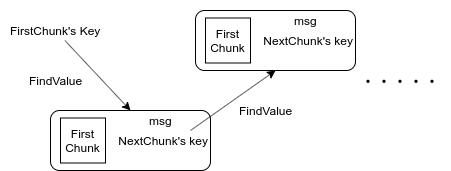
\includegraphics[width=10cm]{./assets/image/subscribeStream.png}
	\caption{ストリームデータの探索}
	\label{fig:subscribe-stream}
\end{figure}

\section{メタデータ}
LayeredKadでは静的, 動的の両方のデータ形式の
共有に対応するために共有するデータの情報メタデータとして
共有し, メタデータの情報に従ってノードの振る舞いを変化させる.
メタデータの基本構造は次のようになっている.
\\
\begin{lstlisting}
type Meta = {
  type: "static" | "stream";
  name: string;
  payload: { [key: string]: any };
};
\end{lstlisting}

typeはメタデータの種類を表す.
本論文ではstaticとstreamの二種類が存在する.

nameはメタデータの名前である. nameには任意の文字列を与える.

payloadには実体データに関する情報を与える.
\\\\
本研究ではこの基本的なMetaデータ構造を拡張したStaticMetaと
StreamMetaが存在する

\subsection{StaticMeta}
静的なデータを扱うメタデータである.
\\
\begin{lstlisting}
type StaticMeta = Meta & {
  type: "static";
  payload: { keys: string[] };
};
\end{lstlisting}

payloadのkeysが実体データのハッシュキーの集合である.
実体データをSubNetで探索する際には, keysのそれぞれのKeyをFindValueで
探索し, 最後に結合する.

\subsection{StreamMeta}
ストリーム(ライブ映像など)を扱うメタデータである.
\\
\begin{lstlisting}
type StreamMetaPayload = {
  first: string;
  width?: number;
  height?: number;
  cycle: number;
};	
type StreamMeta = Meta & {
  type: "stream";
  payload: StreamMetaPayload;
};  
\end{lstlisting}

payloadのfirstが実体データのストリームデータの
最初のチャンクのハッシュキーである.
width, heightは動画の縦横のピクセル数である.
cycleには "$ 1000 \div フレームレート $" の値を与える.
実体データをSubNetで探索する際には, payloadのfirstをFirstChunkのKeyとし, 
\ref{sec:subscribe-stream}節のストリームデータの探索方法に従い, 
ストリームデータをサブスクライブする.

\section{Network}
LayeredKadではネットワークがMainNetとSubNetの2階層存在する.

\subsection{MainNet}
Kademliaをベースとしたネットワークである.
ここでメタデータのやり取りと, 
メタデータの実体データを扱いたいノードとSubNetとの橋渡しを行う.
MainNetのインスタンスは一つのノードにつき一つのみ存在する.

\subsubsection{ノードの種類}
LayeredKadはウェブブラウザのような公開された
トランスポートアドレス\footnote{IPアドレスとポートのペア}
を持たないクライアントデバイスとサーバのような
公開トランスポートアドレスを持つデバイスの両方で動作することを目的としている.
ここでは公開トランスポートアドレスを持たないノードをGuestNodeと呼び, 
公開トランスポートアドレスを持つノードをPortalNodeと呼ぶ.

\subsubsection{ノードの接続方法}
LayeredKadのMainNetのノード間では最終的にWebRTCで通信を行うが, 
WebRTCは通信を開始するためにシグナリングを行う必要がある.
シグナリングのパターンはPortalNodeとPortalNode, 
GuestNodeとPortalNode, GuestNodeとGuestNodeの
3パターンを考慮する必要がある.

\begin{itemize}
	\item {PortalNodeとPortalNode}\\
	      Portalノード間はトランスポートアドレスが公開されているので, 
	      相手のノードのトランスポートアドレスを知っている前提で, 
	      httpで接続を行い, httpを経由してVanilla Iceでシグナリングを行い, 
	      WebRTCの通信を開始する.
	      WebRTCのpeerをKademliaのk-bucketsで管理し, 
	      Kademliaネットワークを構築する.
	      \\
	\item {GuestNodeとPortalNode}\\
	      GuestNodeは公開トランスポートアドレスを持たないので, 必ず
	      GuestNodeからPortalNodeへ接続を要求する必要がある(逆は不可能).
	      GuestNodeはPortalNodeのトランスポートアドレスを知っている前提で
	      httpで接続を行い, httpを経由してVanilla Iceでシグナリングを行い, 
	      WebRTCの通信を開始する.
	      WebRTCのpeerをKademliaのk-bucketsで管理し, 
	      Kademliaネットワークを構築する.
	      \\
	\item {GuestNodeとGuestNode}\\
	      GuestNodeは公開トランスポートアドレスを持たないので, 
	      GuestNode同士で独立して接続を開始することは出来ない.
	      そのため, GuestNode同士が接続されるパターンとして
	      MainNetにWebRTCでの接続を開始(1か2のパターンで)した後に
	      Kademliaのアルゴリズムに従い, 接続されるケースが想定される.
\end{itemize}

ノード間の接続完了後はネットワーク全体で全ノードがWebRTCを用いて共通のプロトコルで
通信するので, あとはKademliaの仕組みに従う.

\subsubsection{MainNetの命令}
MainNetにはStore, FindValue, DeleteValueの3つの命令が定義されている.

\begin{itemize}
	\item {Store}\\
	      MainNet上にメタデータを保存する命令である.
	      \\\\
	      Storeの型定義を以下に示す.
	      \begin{lstlisting}
	type Store = (meta: Meta) => 
		Promise<{ url: string, peers: Peer[] }>
	      \end{lstlisting}
	      	      
	      Storeはメタデータを引数として実行する.
	      実行結果としてメタデータが保存されたアドレス(url)と
	      メタデータを受け取ったノードらの情報(peers)を返す.
	      \\
	\item {FindValue}\\
	      urlに対応するメタデータを探す命令である.
	      \\\\
	      FindValueの型定義を以下に示す.
	      \begin{lstlisting}
	type Store = (url: string) => 
		Promise<{ meta: Meta, peer: Peer }>
	      \end{lstlisting}
	      	      
	      FindValueはurl文字列を引数として実行する.
	      実行結果としてメタデータ(meta)と, 
	      そのメタデータを返してきたノードの情報(peer)を返す.
	      \\
	\item {DeleteData}\\
	      自身の持つメタデータを削除する命令である.
	      \\\\
	      DeleteDataの型定義を以下に示す.
	      \begin{lstlisting}
	type Store = (url: string) => void
	      \end{lstlisting}
	      	      
	      DeleteDataはurl文字列を引数として実行する.
\end{itemize}

\subsection{SubNet}
Kademliaをベースとしたネットワークである.
メタデータの指し示すデータのやり取りを行う.
構造としては, 一つのMainNet上に複数のSubNetが存在することになる.
そのため, SubNetのインスタンスは一つのノードに複数存在しうる.

\subsubsection{ノードの種類}
SubNetはMainNet上で動作するので, すべての通信にWebRTCを使用している.
そのためMainNetと違い, 通信方法によるノードの分類は存在しない.

\subsubsection{SubNetの命令}
SubNetにはFindStaticMetaTargetとFindStreamMetaTargetの2種類の
命令が定義されている.
\begin{itemize}
	\item {FindStaticMetaTarget}\\
	      静的なデータを扱うメタデータの実体データを探索する命令である.
	      \\\\
	      型定義を以下に示す.
	      \begin{lstlisting}
	type FindStaticMetaTarget = () => Promise<ArrayBuffer | undefined>
	      \end{lstlisting}
	      SubNetの持つメタデータを元に実体データを探索し, 
	      探索結果を返す.
	      \\
	\item {FindStreamMetaTarget}\\
	      StreamMetaの実体データを探索する命令である.
	      \\\\
	      型定義を以下に示す.
	      \begin{lstlisting}
	type FindStaticMetaTarget = (
		cb: (res: {
				type: "error" | "chunk" | "complete";
				chunk?: ArrayBuffer;
				}) => void
		) => void
	      \end{lstlisting}
	      SubNetの持つメタデータを元にストリームデータをサブスクライブする.
	      チャンクデータのアノテーションから
	      次にFindValueすべきkeyを入手している.
	      	      	
	      ストリームデータは長さが不明なので終了を持ち受けるのではなく, 
	      入手したチャンクを都度コールバックで渡す.
\end{itemize}

\section{Actor}
ActorはMainNetとSubNetを利用し, 
LayeredKadのシステムを実現するためのノードの実装である.
本論文ではUser, Seeder, Navigatorの3つのActorが存在する.
一つのノードは同時に複数のActorになりうる.

\subsection{User}
Userはデータの探索を行うActorである.
UserはメタデータのURLをもとにMainNet上でメタデータを探索し, 
メタデータを持つNavigatorを仲介してSubNetと接続する.
SubNetと接続しているUserを特にObserveUserと呼ぶ.
また, ObserveUserはSeederの役割を兼ねる.

Userのインスタンスは一つのノードにつき一つのみ存在する.

\subsubsection{SubNetへの接続}
詳細なSubNetへの接続手順を示す.
\begin{enumerate}
	\item メタデータのURLをもとにMainNetでメタデータを探索する
	\item メタデータを返したノード(Navigator)にSeederへの接続仲介を要請する
	\item Seederとの接続完了はSubNetへ接続できたことを意味する
	\item 
	      ObserveUserはSeederのインスタンスを生成し, 接続しているSubNet
	      におけるSeederを兼任する
	\item SeederはNavigatorを兼任するため, 
		  UserはNavigatorのインスタンスも生成する
\end{enumerate}

\subsubsection{Userの命令}
Userには1種類の命令が定義されている.
\begin{itemize}
	\item {ConnectSubNet}\\
	      urlを元にMainNet上でメタデータを探索し, メタデータを
	      返したノードをNavigatorとしてメタデータの実体データを
	      持つ, SeederのSubNetへ接続する.\\
	      	      	      	      
	      型定義を以下に示す.
	      \begin{lstlisting}
	type ConnectSubNet = (url: string) =>
		Promise<{subNet: SubNet, meta:Meta}>
	      \end{lstlisting}
	      	      	      	      
	      メタデータのurlを受け取り, 
	      SubNetとメタデータを返す.
\end{itemize}

UserはConnectSubNetによって接続したSubNetに対して
FindStaticMetaTargetやFindStreamMetaTargetを行うことによって
メタデータの実体データを探索し入手することができる.

\subsection{Seeder}
Seederとはデータの配信を行うActorである.
実際のユースケースでいうところのデータのアップロード者などにあたる.
Seederは任意のデータをもとにメタデータを作成し, 
メタデータをMainNet上にStoreし, SubNetを生成する.

SeederによってMainNet上でメタデータをStoreされたノードはNavigatorとなり, 
SubNetへの接続を要求するUserとSeederの橋渡しを担う.
また, SeederもNavigatorとして振る舞う.

UserがSubNet内でメタデータの実体データを探索する際にSeederは
実体データを所持している場合, そのデータをUserに渡す.
(なお, このプロセスはKademliaのFindValueに従う)

SeederはSubNet毎に存在するので, Seederのインスタンスは
一つのノードに複数存在しうる.

\subsubsection{SubNetの生成}
SeederはメタデータをMainNetにStoreし, その結果
メタデータのurlとStore先のノード情報(peers)を得る.
そしてSeederはメタデータの情報を持ったSubNetを生成し
peersの対象のノードたちをNavigatorにする.

\subsubsection{Seederの命令}
SeederにはStoreStaticとStoreStreamの2種類の命令が定義されている.
\begin{itemize}
	\item{StoreStatic} \\
	静的なデータからメタデータを生成しMainNetに保存する.
	その後メタデータに対応するSubNetを生成し, 
	メタデータの実体データをSubNetに保存する.\\\\					
	型定義を以下に示す.
	\begin{lstlisting}
	type StoreStatic = (name: string, ab: Buffer) =>
		Promise<{url: string, meta: Meta}>
	\end{lstlisting}
					
	引数にメタデータの名前となる文字列と静的なデータを受け取る.
	メタデータのurlとメタデータを返す.
	\\
	\item {StoreStream}\\
	      ストリームデータからメタデータを生成しMainNetに保存する.
	      その後メタデータに対応するSubNetを生成し, 
		  メタデータの実体であるストリームのチャンクデータを
		  SubNetに動的に保存する.\\\\		  
	      型定義を以下に示す.
	      \begin{lstlisting}
	type StoreStream = 
		(name: string, first: Buffer, payload:
			{width:number, heigh:number, cycle:number}
		) => Promise<{event:Trigger, url:string}>
	      \end{lstlisting}

	      引数にメタデータの名前となる文字列と
	      ストリームデータの最初のチャンクデータと
	      ストリームデータの情報を受け取る.
	      戻り値のTriggerはfirstチャンク以降のチャンクデータを送るための
	      コンポーネントである. urlはメタデータのurlである.
\end{itemize}

\subsection{Navigator}
NavigatorはUserをSubNetに接続する際の仲介を行うActorである.
MainNetを監視しており, UserからConnectSubNet命令を受け取った時に, 
Navigatorと接続されたSeederとUserの接続を仲介する.

Navigatorは自分の所持しているメタデータ毎に存在するので, 
Navigatorのインスタンスは一つのノードに複数存在しうる.
NavigatorはSubNetには参加していない.

\subsubsection{Seederとの接続}
LayeredKadのノードはMainNet上でメタデータをStoreされると, 
Navigatorになるので, すべてのノードが潜在的にNavigatorになるうる.
そこで, これからNavigatorになるノードのことをNavigatorCandidateと表現する.
NavigatorCandidateはMainNetを監視しており, 
NavigatorCandidate自らにメタデータをStoreされた時に, 
Storeしてきたノード(Seeder)に対してシグナリングを行い
WebRTCのpeerを生成しコネクションを作る.
これによりNavigatorCandidateはNavigatorとなる.

\subsubsection{UserとSeederの接続仲介}
NavigatorはMainNetを監視し, 
UserがNavigator自らの持つメタデータを探索によって発見し, 
SubNetへの接続要求であるConnectSubNet命令を実行した際に
Navigator自らの接続するSeederに対してUserとの
接続を行うための情報を要求する(WebRTCのSDP等).
その情報をUserへ返し, 次にUserの接続情報(SDP等)をSeederへ渡す.
これによりUserとSeederの間にWebRTCのpeerが生成され接続が完了する.
SeederはSubNet環境下に存在するので, 
Userはメタデータに対応するSubNetに接続できたことになる.

\section{動作}
LayeredKad上で実際にデータを共有するケースの流れについて確認し, 
LayeredKadの動作を確認する.

\subsection{webブラウザから静的なデータを共有する}
\subsubsection{静的データの保存}
\begin{enumerate}
	\item 
	      webブラウザはGuestNodeにあたるので, Portalノードの
	      トランスポートアドレスを何らかの方法で入手し, PortalNodeと接続し, 
	      MainNetにアクセスする.
	      \\
	\item
	      webブラウザはActorのSeederとしてStoreStatic命令を実行し, 
	      メタデータをMainNetに保存し, SubNetを生成し, Navigatorと接続する.
\end{enumerate}
\subsubsection{静的データの探索}
\begin{enumerate}
	\item 
	      webブラウザはGuestNodeにあたるので, Portalノードの
	      トランスポートアドレスを何らかの方法で入手し, PortalNodeと接続し, 
	      MainNetにアクセスする.
	      \\
	\item
	      webブラウザはActorのUserとしてConnectSubNet命令を実行し, 
	      Navigatorを経由してSeederのSubNetへ接続する.
	      \\
	\item 
	      webブラウザはSubNetのFindStaticMetaTarget命令を実行し, 
	      SubNet上でメタデータの実体データを探索し, 入手する.
\end{enumerate}

\subsection{webブラウザかストリームデータを共有する}
\subsubsection{ストリームデータの保存}
\begin{enumerate}
	\item 
	      webブラウザはGuestNodeにあたるので, Portalノードの
	      トランスポートアドレスを何らかの方法で入手し, PortalNodeと接続し, 
	      MainNetにアクセスする
	      \\
	\item
	      webブラウザはActorのSeederとしてStoreStream命令を実行し, 
	      メタデータをMainNetに保存し, SubNetを生成し, Navigatorと接続する.
	      ストリームのチャンクデータを順次Triggerから送信する.	
\end{enumerate}
\subsubsection{ストリームデータの観測}
\begin{enumerate}
	\item 
	      webブラウザはGuestNodeにあたるので, Portalノードの
	      トランスポートアドレスを何らかの方法で入手し, PortalNodeと接続し, 
	      MainNetにアクセスする
	      \\
	\item
	      webブラウザはActorのUserとしてConnectSubNet命令を実行し, 
	      Navigatorを経由してSeederのSubNetへ接続する.
	      \\
	\item 
	      webブラウザはSubNetのFindStreamMetaTarget命令を実行し, 
	      SubNet上でメタデータのペイロードに記載されている
	      firstチャンクデータの実体データを探索し, 入手する.
		  あとは\ref{sec:subscribe-stream}節のようにmsgアノテーション
		  を辿りチャンクの探索を続けることでストリームデータの観測を行う.
\end{enumerate}

\section{実装}
すべての実装において, 使用したプログラム言語はTypeScriptである.

\subsection{ライブラリ}
Node.jsとwebブラウザ上で動作するように実装を行った.
P2P通信部部にはWebRTCを用いている.

\subsection{ベンチマーカー}
通常のKademliaとLayeredKadの性能比較を行うために, 
Node.js上で動作するベンチマーカーの実装を行った.
なお, ベンチマーカーは実装の都合上P2P通信部分はWebRTCではなく, 
UDPを使用してWebRTCの挙動を再現している.

\subsection{サンプルプログラム}
実際にwebブラウザ上でLayeredKadを用いてライブストリーミングの
配信と視聴を行うサンプルプログラムを作成した.
Webのフロントエンド部分はReact\footnote{https://reactjs.org/}
を使用した.P2P通信部部にはブラウザ搭載のWebRTCを用いている.

動作確認の結果, ローカル環境下で数ノード(5ノード以上)のLayeredKadネットワーク
を構築した状況ではライブストリーミングの配信/視聴が可能であることを
確認できた.

% ---------------------------------------------------------------------
\chapter{評価実験}
本論文では, データ通信量と, タスクの処理時間の2つの観点から, 
LayeredKadの評価を行う.
本実験では, 現実的なユースケースとして, 
幾つかのファイルがネットワーク上に共有され, 
それぞれのファイルに関心があるユーザがそれぞれのデータ毎にグループを形成し
共有しあっているケースを想定し仮説を立て, 実験検証を行う.
評価実験のシナリオのイメージを
図\ref{fig:trafficBenchmark}に示す.

\begin{figure}[H]
	\centering
	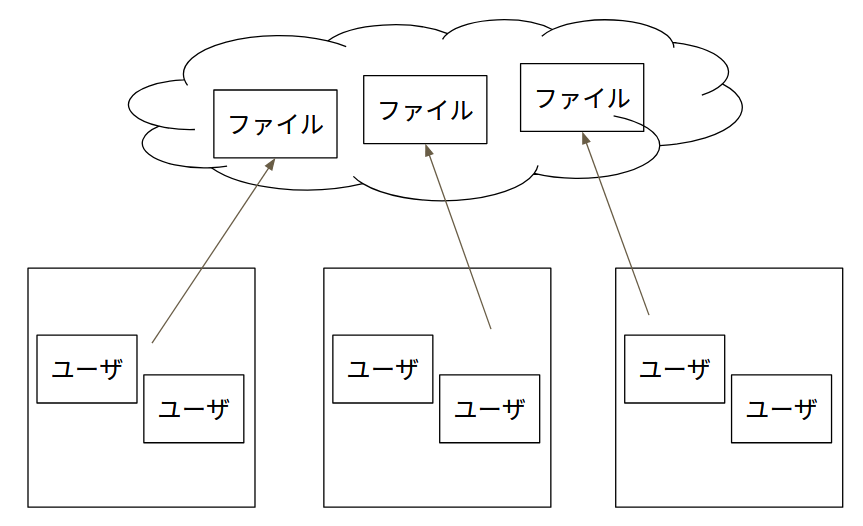
\includegraphics[width=10cm]{./assets/image/traffic_benchmark.png}
	\caption{評価実験のシナリオのイメージ}
	\label{fig:trafficBenchmark}
\end{figure}

\section{データ通信量}
\subsection{仮説}
LayeredKadでは共有するデータごとにネットワークを分割しており, 
データの保存や探索がネットワーク全体に影響しないので, 
Kademliaとノード数が同じであれば, ネットワーク全体における, 
データ通信量が少なくなることが予想される.
ファイル共有サービスにおいてファイル共有速度の最も大きな
ボトルネックはネットワークの通信速度であり, 
特にライブストリーミングデータは大容量なデータを高頻度に
やり取りする必要があるため, 
データ通信量が少ないことは大きなメリットである.

\subsection{実験}
\subsubsection{実験方法}
データ通信量の計測を行うために, KademliaとLayeredKadで
データ通信量の計測を行うベンチマークプログラムを作成した.
ベンチマークプログラムは表\ref{table:spec-note}の環境で実行した.

\begin{table}[H]
	\caption{スペック}	
	\centering
	\label{table:spec-note}
	\begin{tabular}{|l|l|}
		\hline
		CPU &   
		Intel Core i7-7500U 2.70GHz 2Core 4Threads\\ 
		\hline	
		OS  &   
		Ubuntu 19.10 \\ 
		\hline
	\end{tabular}	
\end{table}

本ベンチマークプログラムでは, ノードのペアを1グループとして, 
ファイル共有を行わせる.
ノード数を変数パラメータとして, パラメータの値を増加させ, 
LayeredKadとKademliaのデータ通信回数を記録し, 比較を行う.

\subsubsection{実験結果}
KademliaとLayeredKadの実験結果の表を表\ref{table:traffic-result}に

Kademliaの実験結果のグラフを図\ref{figure:traffic-1}に, 

LayeredKadの実験結果のグラフを図\ref{figure:traffic-2}に, 

KademliaとLayeredKadの実験結果のグラフを\ref{figure:traffic-3}に示す.

\begin{table}[H]
	\caption{KademliaとLayeredKadの実験結果}
	\centering
	\label{table:traffic-result}
	\begin{tabular}{|l|l|l|}
		\hline
		ノード数   &   
		Kademlia (回) &   
		LayeredKad (回)\\
		\hline
		10             &   
		90             &   
		5\\
		\hline
		20             &   
		380            &   
		10\\
		\hline
		30             &   
		600            &   
		16\\
		\hline
		40             &   
		779            &   
		26\\
		\hline
		50             &   
		965            &   
		36\\
		\hline
		60             &   
		1132           &   
		48\\
		\hline
	\end{tabular}
\end{table}

\begin{figure}[H]
	\centering
	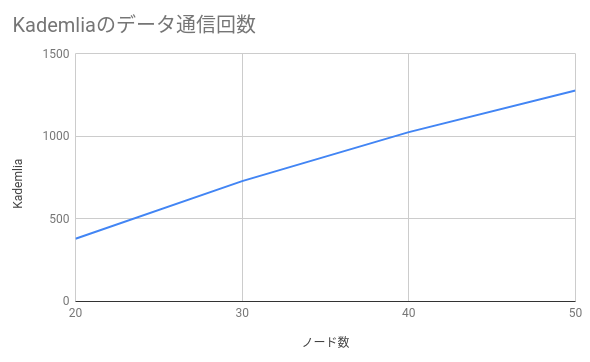
\includegraphics[width=10cm]{./assets/image/kad_traffic.png}
	\caption{kademliaの通信量}
	\label{figure:traffic-1}
\end{figure}

\begin{figure}[H]
	\centering
	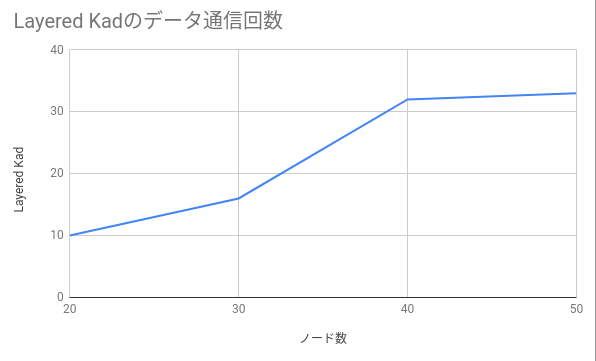
\includegraphics[width=10cm]{./assets/image/layered-kad_traffic.png}
	\caption{layeredKadの通信量}
	\label{figure:traffic-2}
\end{figure}

\begin{figure}[H]	
	\centering
	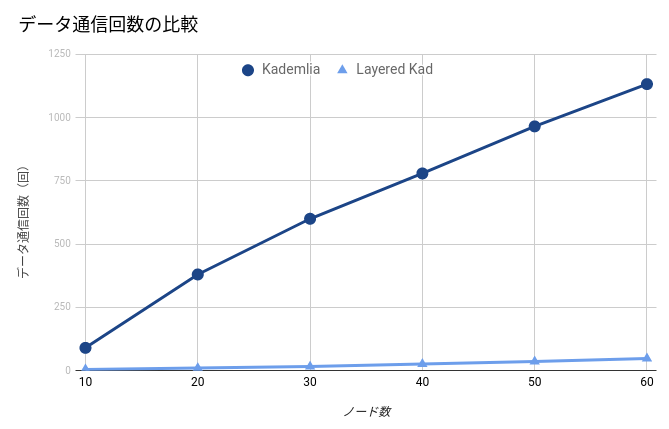
\includegraphics[width=10cm]{./assets/image/traffic_graph.png}
	\caption{通信量の比較}
	\label{figure:traffic-3}
\end{figure}

ノード数がいずれの場合においても, データ通信回数はLayeredKadがKademlia
を大きく下回った.

\subsection{考察}
実験結果は, 仮説の通りの結果となった.
Kademliaは一つのデータを保存する際に, 
k-bucketのサイズ分(本論文では20)のノードとデータのやり取りを
することになるため, この実験結果のような通信回数になったと考えられる.

一方LayeredKadはデータ毎にSubNetを生成し, その内部でデータの
やり取りを行うため, 本実験の場合データをノードのペアがやり取りを行う
シナリオとなっているためSubNetにはノードが2つしか無く, 
データのやり取りは1回で済む.
そのため, Kademliaより通信回数が大幅に少なくなったと考えられる.

\section{タスクの処理時間}
\subsection{仮説}
LayeredKadはKademliaをさらに構造化したシステムであるため, 
単純に一つのデータをネットワーク全体で共有するようなケースでは, 
処理のステップ数の少ないKademliaの方が高速であると予想される.
しかし今回の実験ケースでは複数のデータを複数のユーザグループ毎に
共有しているので, Kademliaはすべてのデータにおける
処理をネットワーク全体で行う必要があるのに対して, 
LayeredKadではユーザグループ(SubNet)内で完結するため, 
処理効率がよくタスクの処理時間も短くなると考えられる.

\subsection{実験}
\subsubsection{実験方法}
タスク処理時間の計測を行うために, KademliaとLayeredKadで
タスク処理時間の計測を行うベンチマークプログラムを作成した.
ベンチマークプログラムは表\ref{table:spec-ryzen}の環境で実行した.

\begin{table}[H]
	\caption{スペック}	
	\centering
	\label{table:spec-ryzen}
	\begin{tabular}{|l|l|}
		\hline
		CPU &   
		Ryzen Threadripper 2950X 3.50Ghz 16Core 32Threads \\ 
		\hline	
		OS  &   
		Ubuntu 18.04 \\ 
		\hline
	\end{tabular}	
\end{table}

本実験のシナリオとデータ通信量のベンチマーカーのシナリオとの相違点は
通信量ベンチマーカーがノード数を変数としていたのに対して, 
本実験のベンチマーカーはノード数をノード数を16で固定とし, 
共有するデータ数のチャンキング数を変数としている点である.
ストリームデータはチャンク数が非常に多いので, チャンク数が多いほど
ストリームデータに性質が近いと言える.
タスク処理時間をより正確に計測するために, 
1ノードに付き, CPUのスレッド1つを割り当てるようにベンチマークプログラムの
マルチスレッド化を行っている.

\subsubsection{実験結果}
KademliaとLayeredKadの実験結果を表\ref{table:calc-result}と
図\ref{fig:calc_compare.png}に示す.

\begin{table}[H]
	\caption{実験結果}
	\centering
	\label{table:calc-result}
	\begin{tabular}{|l|l|l|}
		\hline
		チャンク数 &   
		Kademlia (s)    &   
		Layered Kad (s)\\ 
		\hline
		1               &   
		0.636           &   
		2.098\\
		\hline
		2               &   
		0.636           &   
		2.098\\
		\hline
		3               &   
		0.636           &   
		2.098\\
		\hline
		4               &   
		2.032           &   
		2.728\\
		\hline
		5               &   
		2.435           &   
		2.469\\
		\hline
		6               &   
		7.679(2.679)    &   
		2.581\\
		\hline
		7               &   
		13.334(8.334)    &   
		2.581\\
		\hline
		8               &   
		12.679(7.619)    &   
		2.581\\
		\hline
		9               &   
		14.313(9.313)    &   
		2.581\\
		\hline
		10               &   
		13.586(8.586)    &   
		3.635\\
		\hline
	\end{tabular}
\end{table}

\begin{figure}[H]
	\centering
	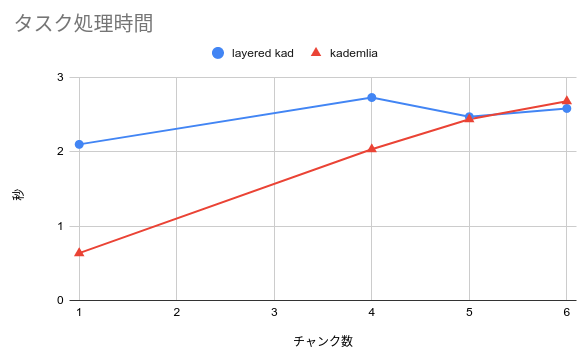
\includegraphics[width=10cm]{./assets/image/calc_compare.png}
	\caption{タスク処理時間の比較}
	\label{fig:calc_compare.png}
\end{figure}

表\ref{table:calc-result}のチャンク数6以降でのKademliaの結果を
"7.679(2.679)"のようにしているのは, Kademliaがこのベンチマークで
タイムアウトを引き起こしていたので, タイムアウトの時間5秒を
引いた値を参考値として括弧の中に表記している.
また, 図\ref{fig:calc_compare.png}のグラフの値は括弧中のものを
使用している.

図\ref{fig:calc_compare.png}のグラフより
Kademliaはチャンク数の増加に比例して, タスク処理時間が増大しているが
LayeredKadはチャンク数の増加が, タスク処理時間にあまり影響していない
ことがわかる.

\subsection{考察}
\subsubsection{Kademliaで発生したタイムアウトの原因}
本ベンチマークでは, 複数のノードが全く同時にデータの共有タスクを
実行しているので, 現実のユースケースより, むしろ高負荷であるため, 
内部でデッドロックが発生してタイムアウトが生じたと考えられる.
本研究のLayeredKadのMainNetとSubNet内部のKademlia実装部分は, 
比較用のKademlia実装とソースコードが同一であるため, 
同一条件下でLayeredKadではタイムアウトが生じていないという点
もLayeredKadの優位性を示せていると考えられる.
\subsubsection{LayeredKadとKademliaの比較}
LayeredKadではデータのチャンキング数が増加しても
タスク処理時間は概ね変化しないのに対して, 
Kademliaではチャンキング数の増加に対してタスク処理時間が比例増大
している原因は
LayeredKadでは, いくらチャンク数が増えたとしてもSubNetのペアとなるノードとの
一対一の通信回数がチャンク数分増えるだけなのに対して, 
Kademliaはチャンク数分, ネットワーク全体に対して問い合わせるため, 
その分処理時間が増大しているからだと考えられる.

% ---------------------------------------------------------------------

\chapter{おわりに}
\section{結論}
本論文では, Kademliaをベースに効率的にストリーム形式の
データを共有できるシステムの開発を行った.
ネットワークを共有するデータ毎に分割し, 非効率的なデータ通信を削減する
仕組みであるLayeredKadを考案し, 実装した.
静的なデータや動的なデータなどを柔軟に扱えるようにするために, 
拡張性の高いメタデータを共有する仕組みを考案した.
メタデータを共有するネットワークをMainNetとし, 
メタデータの実体データを共有するネットワークをSubNetとし, 
ネットワークの分割を実現した.

LayeredKadの性能を評価するため, ユーザが実利用する際のシチュエーション
に沿ったシナリオ上で, LayeredKadとKademliaのベンチマークを行い
性能の評価を行った.
ベンチマークはネットワーク性能のボトルネックとなるデータ通信と, 
タスク処理時間の二項目に着目して行った.
データ通信のベンチマークでは, LayeredKadはそのネットワーク分割能力
によってKademliaよりデータ通信量が小さいごとを実証できた.
タスク処理時間のベンチマークでは, Kademliaがチャンク数の増加に対して
処理時間が比例増大したのに対して, 
LayeredKadではチャンク数の増加が処理時間に影響しないことがわかった.

メタデータによる柔軟なデータ定義, 現実的な特定のユースケースにおける
高パフォーマンスな性能によって, LayeredKadがライブストリーミングに対応した
分散ハッシュテーブルの基盤としての有用であることを示せたと考えられる.

\section{課題}
本研究ではLayeredKadのSubNetのノード数が少ない条件でしか実験が出来ていない.
そのため, SubNetのノード数が増大(Kより大幅に多い数に)した際には
通常のKademliaと同じような問題が発生すると考えられる.
(SubNet内部のネットワーク実装は通常のKademliaと同一であるため.)
この問題を回避する案として, さらにSubNetを分割し構造化するなどといった
アイデアが考えられるが, 本研究では実装の範囲外とした.

\begin{acknowledgment}
	本研究を進めるにあたり, ご指導を頂いた指導教員の萩原助教授に感謝致します.
	日頃の議論において助言や知識を頂いた萩原研究室の皆様に感謝します.
\end{acknowledgment}

\bibliographystyle{unsrt}
\bibliography{reference}
\end{document}